\chapter{Robotic manipulators}\label{chap:robotic-manipulators}

\section*{}

Robotic manipulators have been evolving over the years to fit the automation demand of the industry that needs the ability to move end-effectors with accuracy and speed for performing a wide range of tasks. One of these tasks is robotic assembly operations which require the capability to sense, grasp and move objects of different size, weight and shape within a given work space. The next sections give a brief overview of the main components of robotic manipulators.


\section{Robotic arms}

Robotic arms give the mechanical support for the end effectors (for example grippers, sprayers, grinders, welders, perception sensors, among many others) and can have a wide range of hardware configurations depending on the type of motion that is required for performing a given task. The main categories of robotic arms will be presented in the next sections.


\subsection{Cartesian robotic arms}

Cartesian robots have three linear axis of motion (diagrams shown in \cref{fig:cartesian-robot}) and are used in operations that require mainly translations of the end effector (example in \cref{fig:cartesian-robot-festo-3d-gantry}), such as moving objects within large workplaces or spraying / milling / drilling / cutting material using \glspl{cnc} machines.

\begin{figure}[H]
	\begin{floatrow}[2]
		\ffigbox[\FBwidth]
		{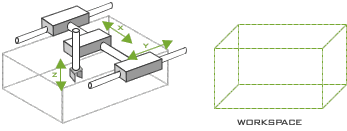
\includegraphics[height=.15\textheight]{robots/cartesian-robot}
		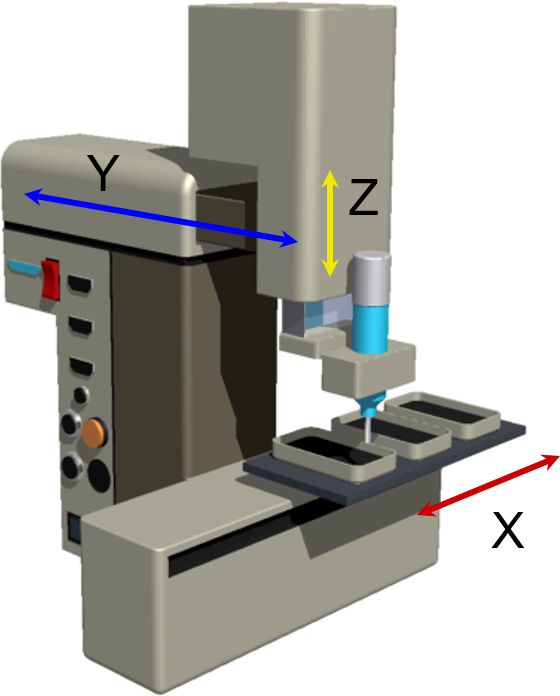
\includegraphics[height=.15\textheight]{robots/cartesian-robot-model}}
		{\caption[Diagrams of a Cartesian robot]{Diagrams of a Cartesian robot\protect\footnotemark}\label{fig:cartesian-robot}}

		\ffigbox[\FBwidth]
		{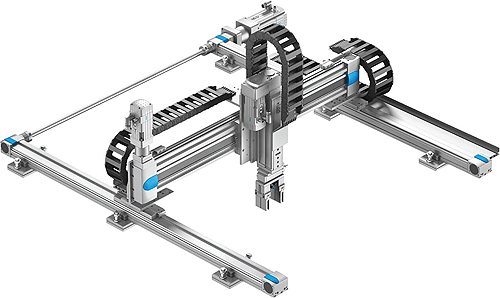
\includegraphics[height=.15\textheight]{robots/cartesian-robot-festo-3d-gantry}}
		{\caption[Cartesian robot with a dual finger gripper]{Cartesian robot with a dual finger gripper\protect\footnotemark}\label{fig:cartesian-robot-festo-3d-gantry}}
	\end{floatrow}
\end{figure}
\footnotetext[\the\numexpr\value{footnote}-1\relax]{\url{http://slideplayer.com/slide/7362200}}
\footnotetext[\value{footnote}]{\url{http://www.linearmotiontips.com/switching-robot-systems-cartesian-handling-systems}}


\subsection{Cylindrical robotic arms}

Cylindrical robots have two linear axis and one rotation axis around the origin (diagrams shown in \cref{fig:cylindrical-robot}) and are useful for tasks such as sorting / packaging (example in \cref{fig:cylindrical-robot-plate-crane}) that require the movement of high payload packages.

\begin{figure}[H]
	\begin{floatrow}[2]
		\ffigbox[\FBwidth]
		{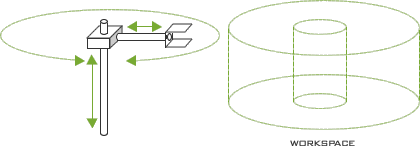
\includegraphics[height=.15\textheight]{robots/cylindrical-robot}
		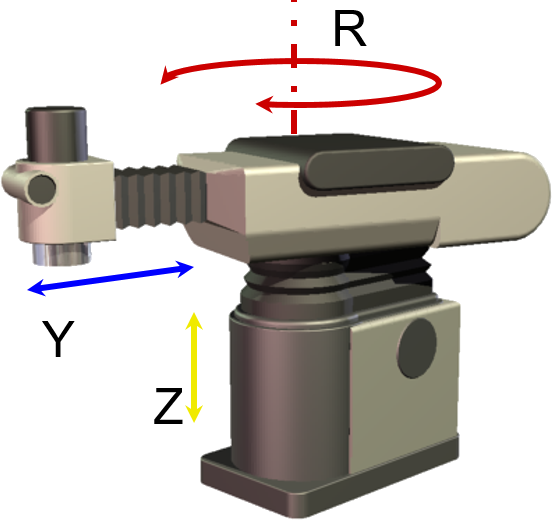
\includegraphics[height=.15\textheight]{robots/cylindrical-robot-model}}
		{\caption[Diagrams of a cylindrical robot]{Diagrams of a cylindrical robot\protect\footnotemark}\label{fig:cylindrical-robot}}

		\ffigbox[\FBwidth]
		{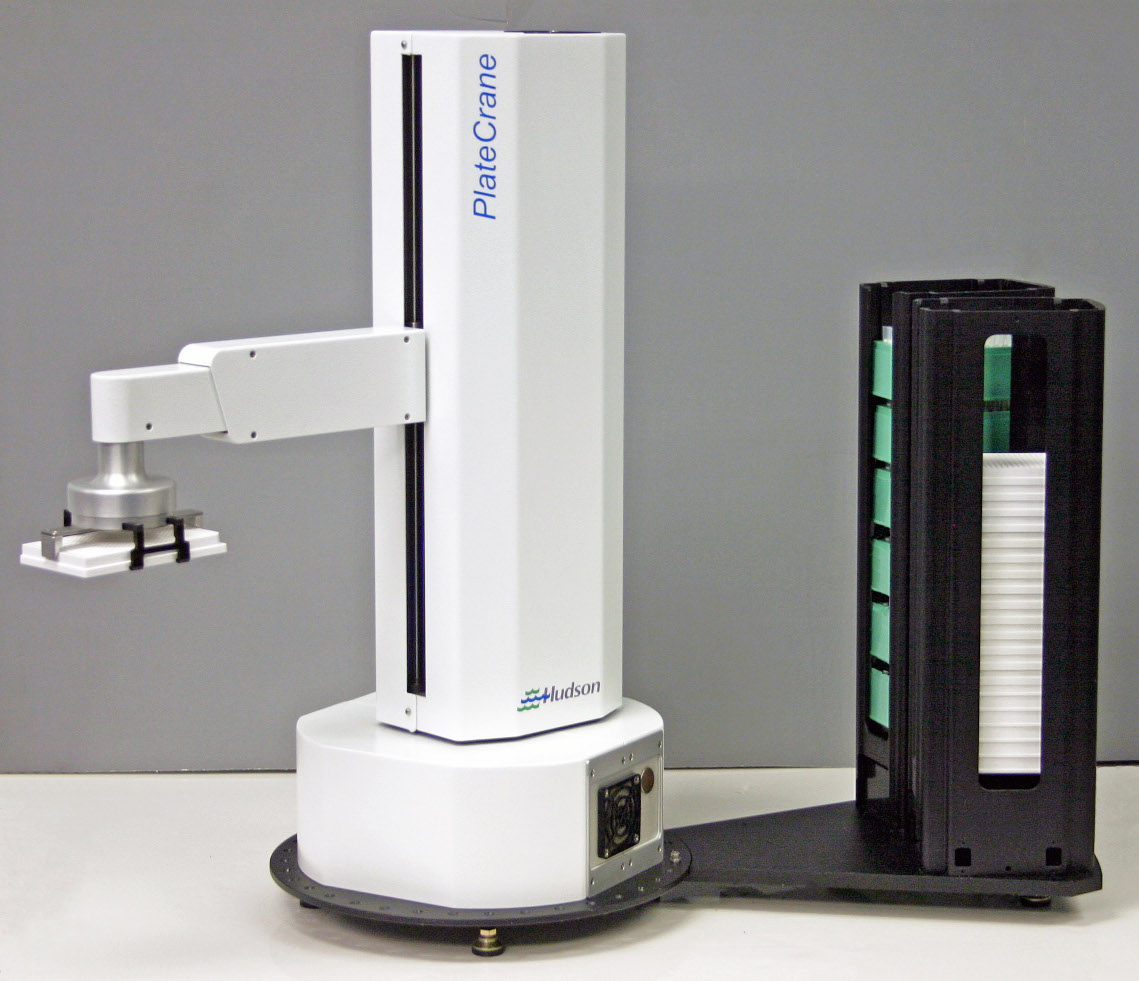
\includegraphics[height=.15\textheight]{robots/cylindrical-robot-plate-crane}}
		{\caption[Cylindrical robot with a dual finger gripper]{Cylindrical robot with a dual finger gripper\protect\footnotemark}\label{fig:cylindrical-robot-plate-crane}}
	\end{floatrow}
\end{figure}
\footnotetext[\the\numexpr\value{footnote}-1\relax]{\url{http://slideplayer.com/slide/7362200}}
\footnotetext[\value{footnote}]{\url{http://hudsonrobotics.com/products/microplate-handling/platecrane-ex}}


\subsection{Polar robotic arms}

Polar / spherical robots have one linear axis and two perpendicular rotation axis (diagrams shown in \cref{fig:polar-robot}) and can be used in welding / fettling operations (example in \cref{fig:polar-robot-fanuc}).

\begin{figure}[H]
	\begin{floatrow}[2]
		\ffigbox[\FBwidth]
		{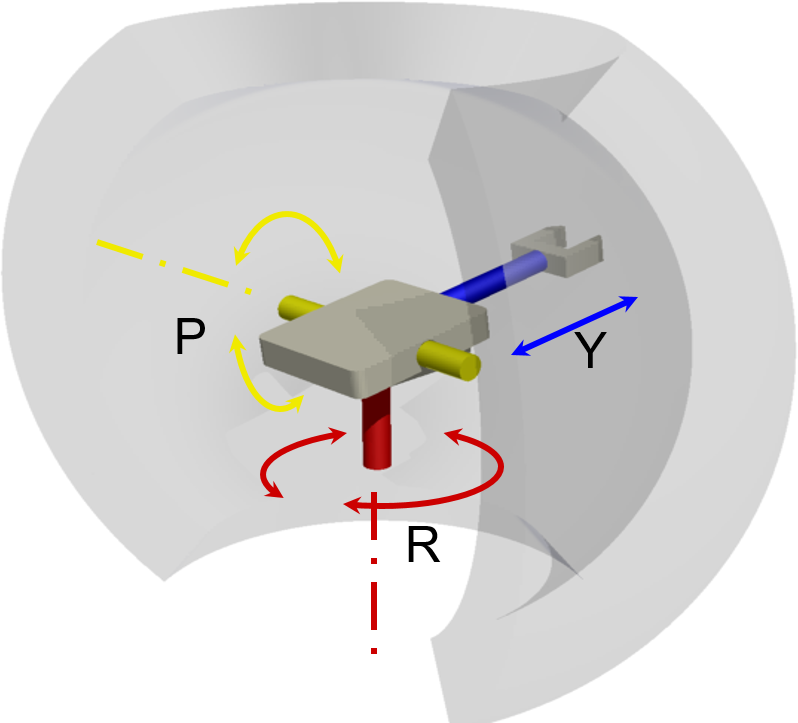
\includegraphics[height=.138\textheight]{robots/polar-robot}
		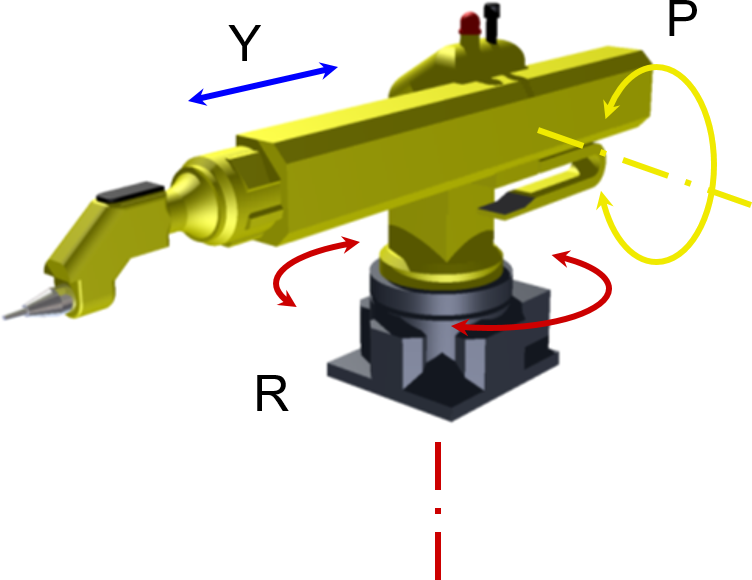
\includegraphics[height=.138\textheight]{robots/polar-robot-model}}
		{\caption[Diagrams of a polar robot]{Diagrams of a polar robot\protect\footnotemark}\label{fig:polar-robot}}

		\ffigbox[\FBwidth]
		{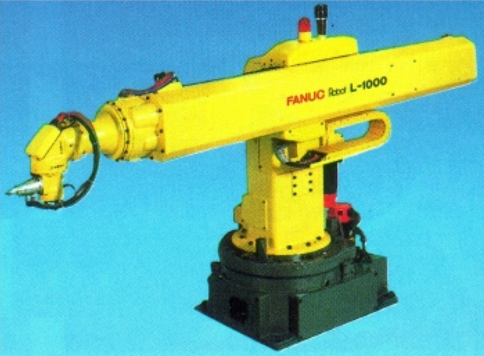
\includegraphics[height=.138\textheight]{robots/polar-robot-fanuc}}
		{\caption[Polar robot]{Polar robot\protect\footnotemark}\label{fig:polar-robot-fanuc}}
	\end{floatrow}
\end{figure}
\footnotetext[\the\numexpr\value{footnote}-1\relax]{\url{http://slideplayer.com/slide/7362200}}
\footnotetext[\value{footnote}]{\url{http://saba.kntu.ac.ir/eecd/ecourses/robotics/overview.pdf}}


\subsection{\glsentrytext{scara} robotic arms}

\gls{scara} robots have one linear axis and two parallel rotation axis (diagrams shown in \cref{fig:scara-robot}) and can perform quick pick and place tasks (example in \cref{fig:scara-robot-packaging}).

\begin{figure}[H]
	\begin{floatrow}[2]
		\ffigbox[\FBwidth]
		{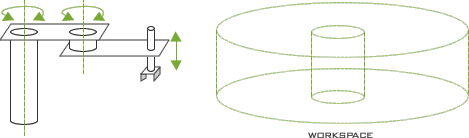
\includegraphics[height=.173\textheight]{robots/scara-robot}
		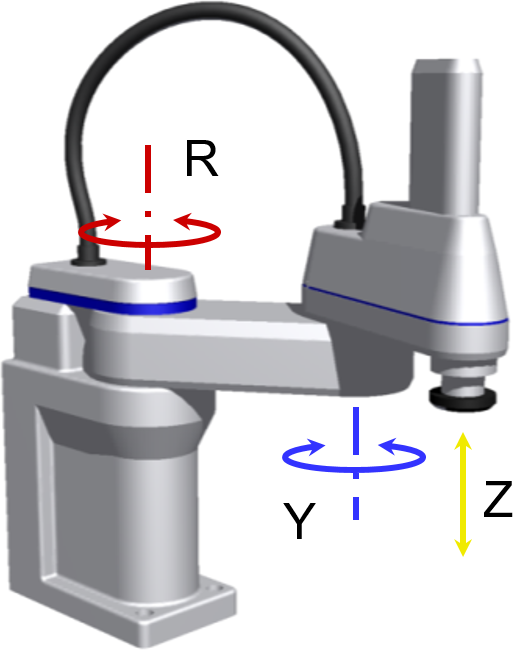
\includegraphics[height=.173\textheight]{robots/scara-robot-model}}
		{\caption[Diagrams of a \glsentrytext{scara} robot]{Diagrams of a \glsentrytext{scara} robot\protect\footnotemark}\label{fig:scara-robot}}

		\ffigbox[\FBwidth]
		{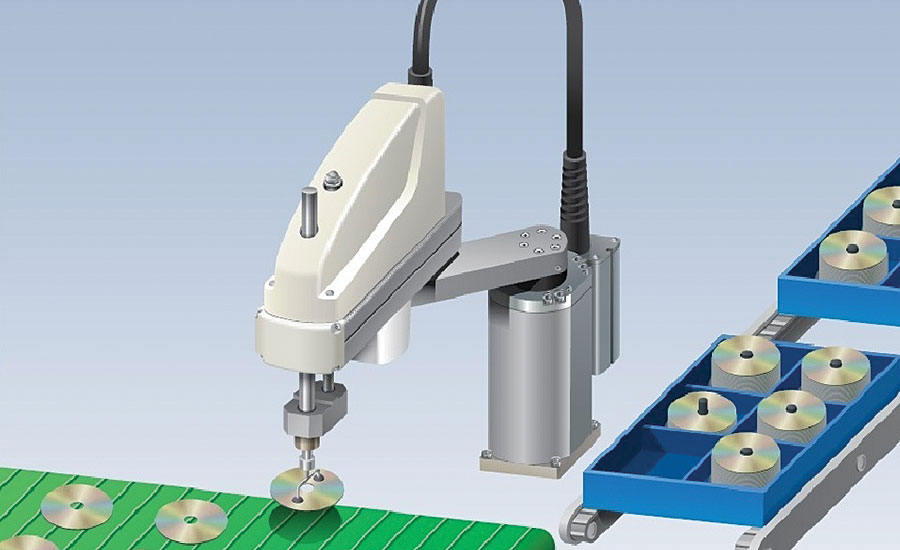
\includegraphics[height=.173\textheight]{robots/scara-robot-packaging}}
		{\caption[\glsentrytext{scara} robot packaging products]{\glsentrytext{scara} robot packaging products\protect\footnotemark}\label{fig:scara-robot-packaging}}
	\end{floatrow}
\end{figure}
\footnotetext[\the\numexpr\value{footnote}-1\relax]{\url{http://slideplayer.com/slide/7362200}}
\footnotetext[\value{footnote}]{\url{http://www.assemblymag.com/articles/93338-whats-new-with-scara-robots}}


\subsection{Parallel / delta robotic arms}

Picker / delta / parallel robots have three parallelogram arms connected to the end effector in order to provide three translation axis and one rotation axis (diagrams shown in \cref{fig:schema-delta-type-1-side-view,fig:paralell-robot-abb}) and they can perform very fast pick and place tasks (example in \cref{fig:picker-parallel-robot-fanuc}).

\begin{figure}[H]
	\begin{floatrow}[3]
		\ffigbox[1.05\FBwidth]
		{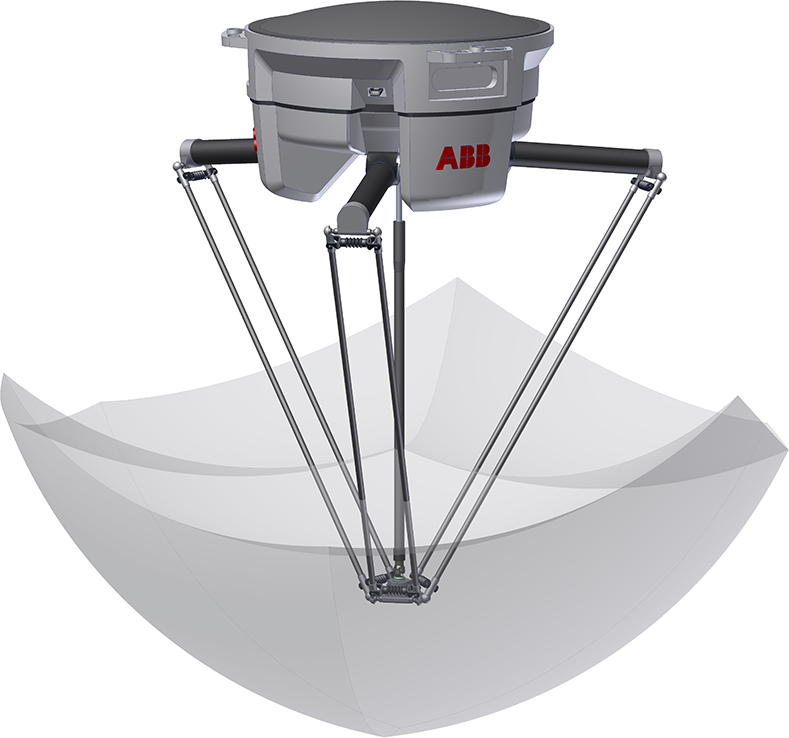
\includegraphics[height=.2\textheight]{robots/paralell-robot-abb}}
		{\caption[Model of a delta robot]{Model of a delta robot\protect\footnotemark}\label{fig:paralell-robot-abb}}

		\ffigbox[\FBwidth]
		{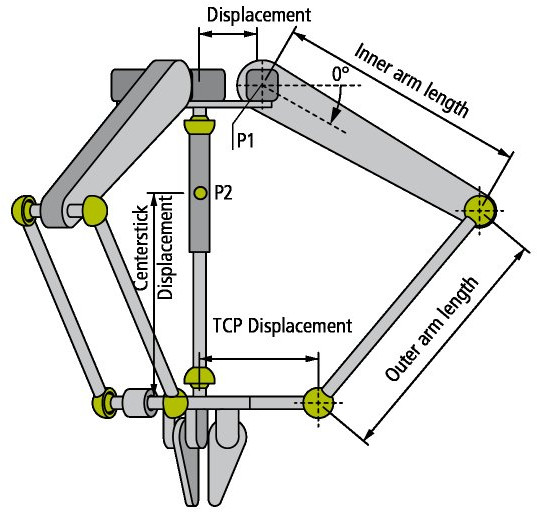
\includegraphics[height=.2\textheight]{robots/schema-delta-type-1-side-view}}
		{\caption[Diagram of a delta robot]{Diagram of a delta robot\protect\footnotemark}\label{fig:schema-delta-type-1-side-view}}

		\ffigbox[\FBwidth]
		{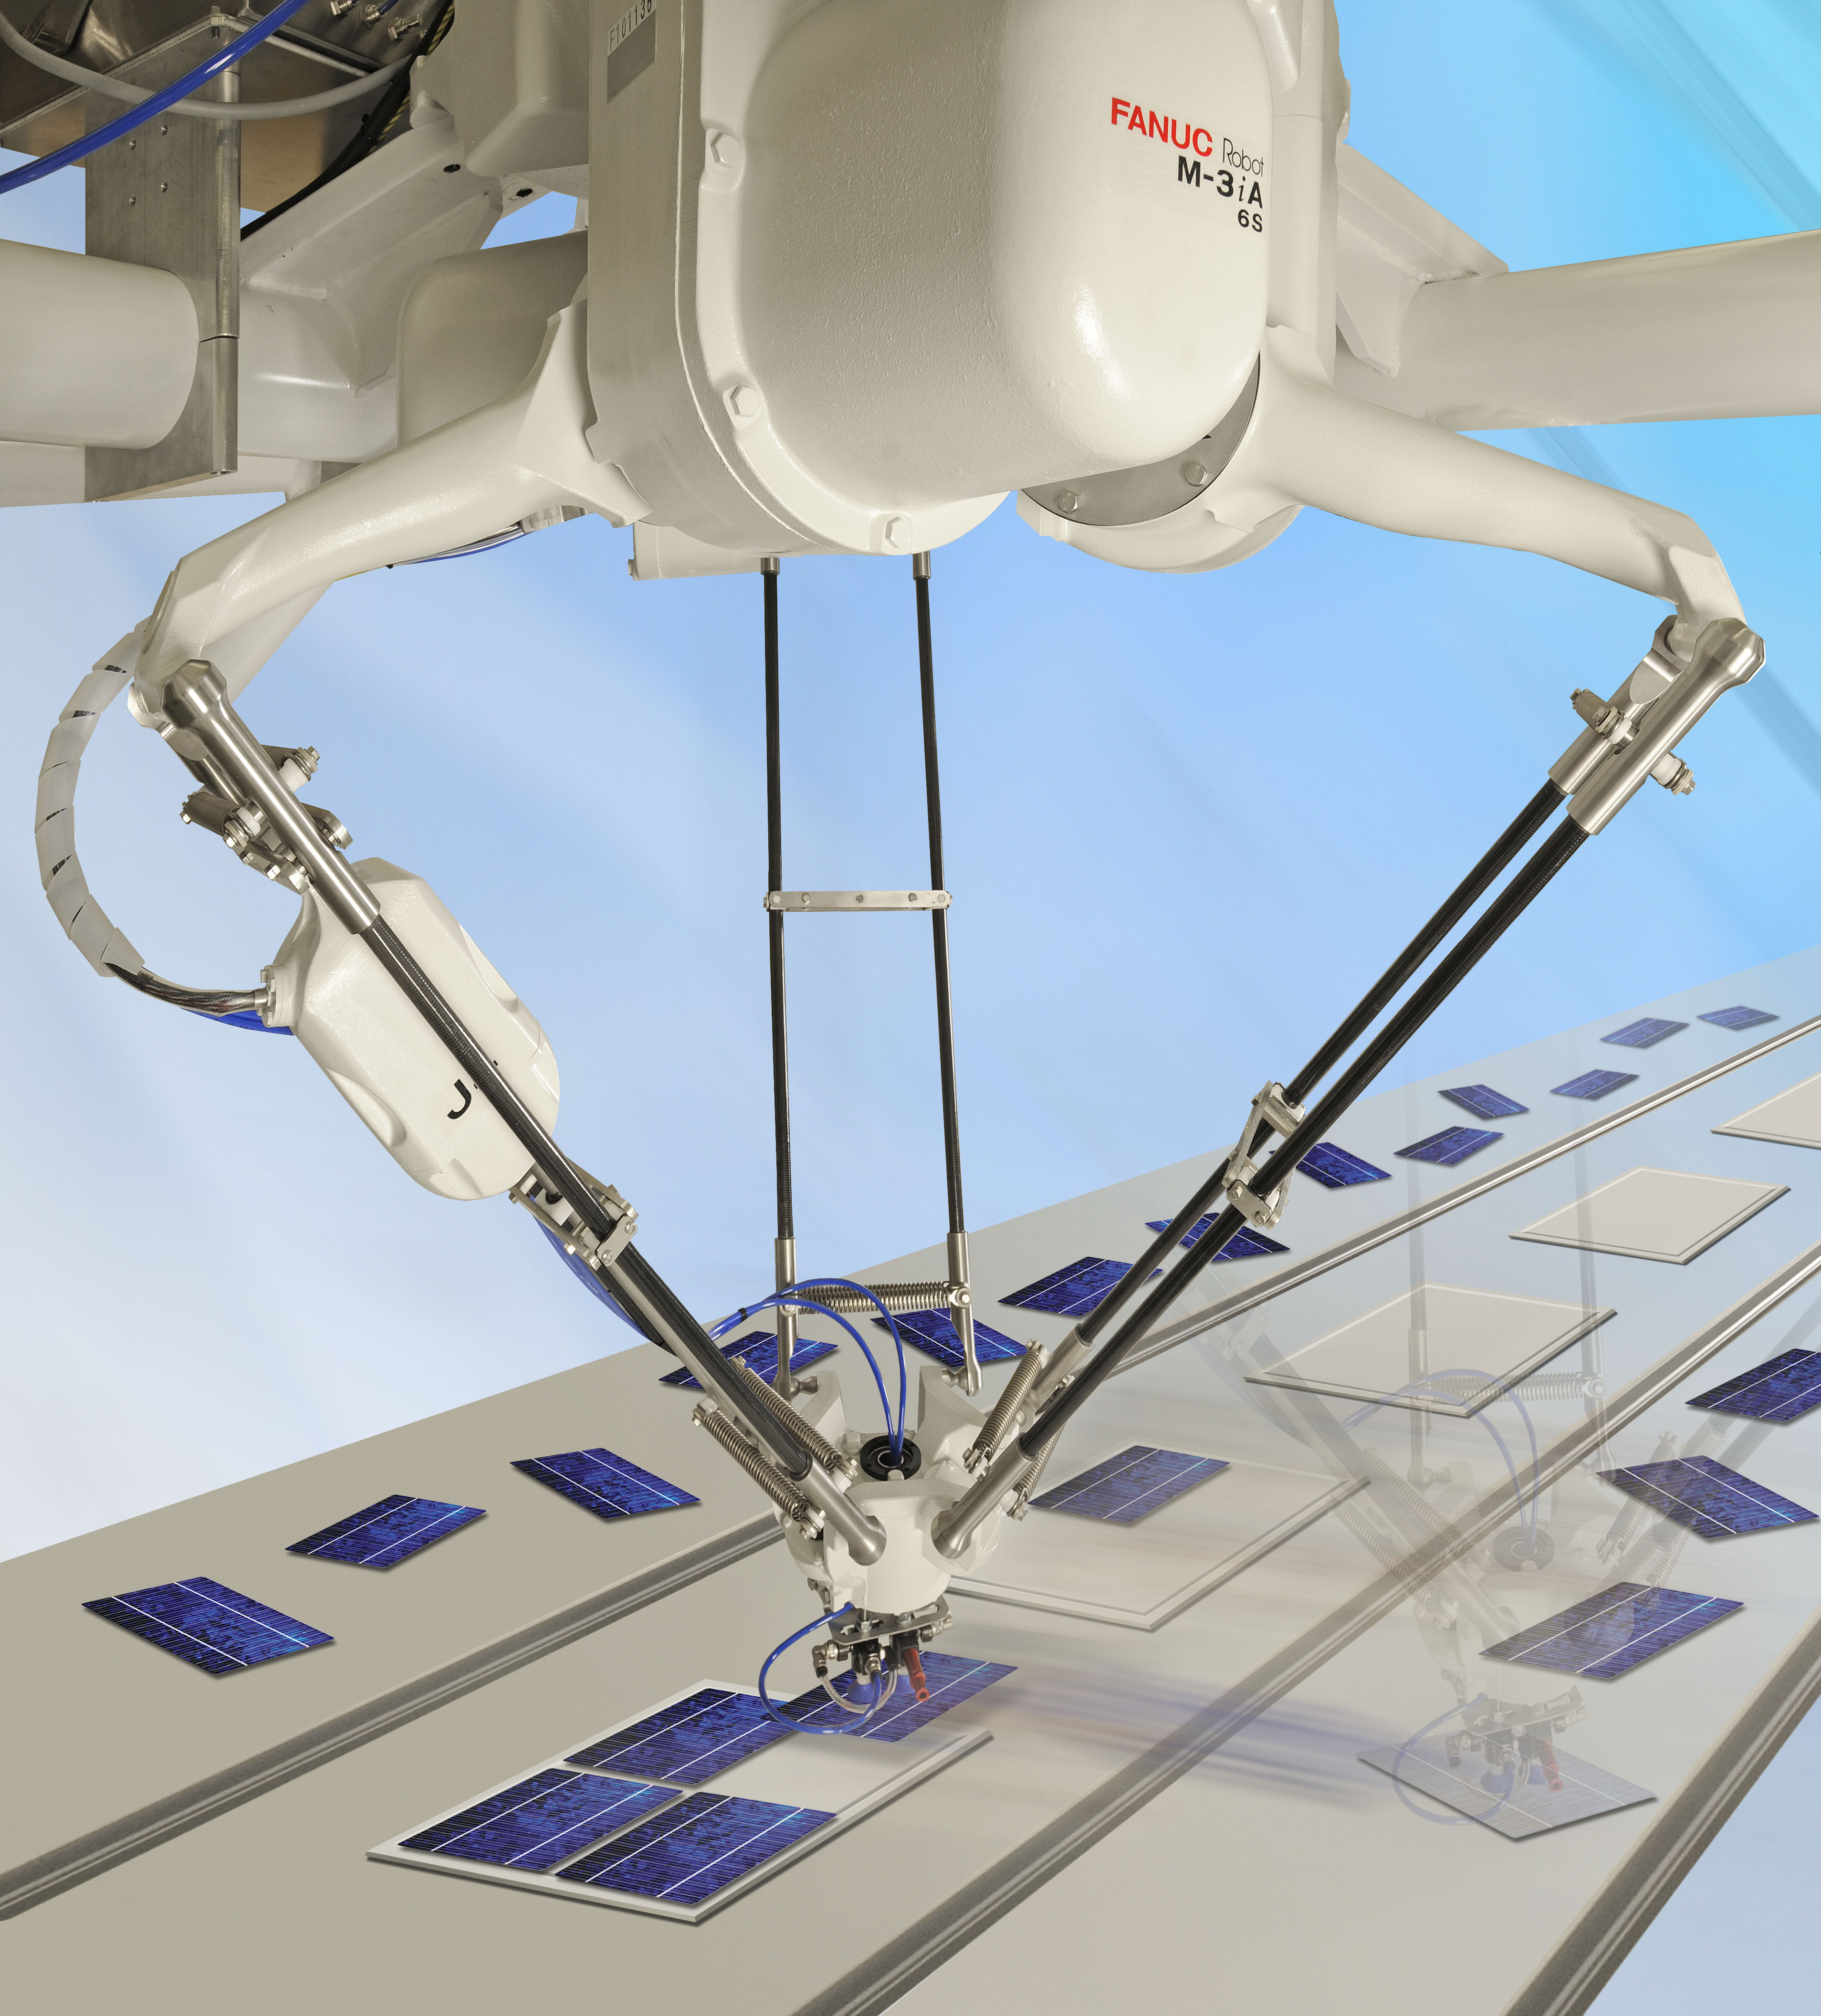
\includegraphics[height=.2\textheight]{robots/picker-parallel-robot-fanuc}}
		{\caption[Delta robot packaging products]{Delta robot packaging products\protect\footnotemark}\label{fig:picker-parallel-robot-fanuc}}
	\end{floatrow}
\end{figure}
\footnotetext[\the\numexpr\value{footnote}-2\relax]{\url{http://www.mecademic.com/What-is-a-parallel-robot.html}}
\footnotetext[\the\numexpr\value{footnote}-1\relax]{\url{http://infosys.beckhoff.com/content/1034/tckintransformation/html/tcnckintransformation_deltatype1.htm?id=21945}}
\footnotetext[\value{footnote}]{\url{http://robot.fanucamerica.com/products/robots/picking-and-packing-robots.aspx}}


\subsection{Snake robotic arms}

Snake robots are flexible manipulators with a high number of interconnected joints (structure of a snake robot shown in \cref{fig:snake-arm-robot-diagram}) capable of bending like a snake in order to access small and difficult to reach areas (example in \cref{fig:laser-snake-pipe-cutting}).


\begin{figure}[H]
	\begin{floatrow}[2]
		\ffigbox[\FBwidth]
		{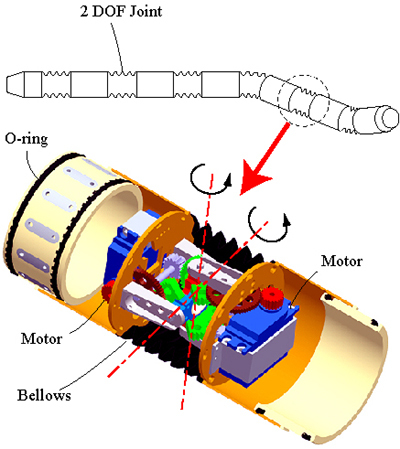
\includegraphics[height=.173\textheight]{robots/snake-robot-diagram}
		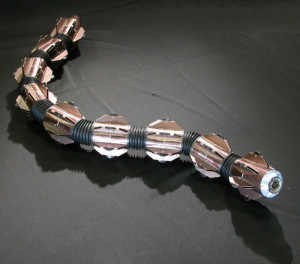
\includegraphics[height=.173\textheight]{robots/snake-robot}}
		{\caption[Structure of a snake robot]{Structure of a snake robot\protect\footnotemark}\label{fig:snake-arm-robot-diagram}}

		\ffigbox[\FBwidth]
		{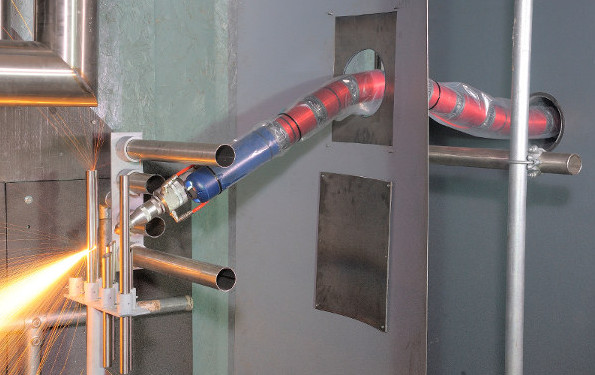
\includegraphics[height=.173\textheight]{robots/laser-snake-pipe-cutting}}
		{\caption[Laser snake robot cutting a pipe]{Laser snake robot cutting a pipe\protect\footnotemark}\label{fig:laser-snake-pipe-cutting}}
	\end{floatrow}
\end{figure}
\footnotetext[\the\numexpr\value{footnote}-1\relax]{\url{https://techcrunch.com/2010/08/18/video-giant-snake-robot-acm-r5}}
\footnotetext[\value{footnote}]{\url{http://sparc-robotics.eu/nuclear-decommissioning}}


\subsection{Articulated robotic arms}

Articulated robots are versatile arms with at least 3 rotation axis (diagrams shown in \cref{fig:articulated-robot}) and are capable of performing a wide range of tasks, from welding to advanced assembly tasks (example in \cref{fig:articulated-robot-kuka}).

\begin{figure}[H]
	\begin{floatrow}[2]
		\ffigbox[\FBwidth]
		{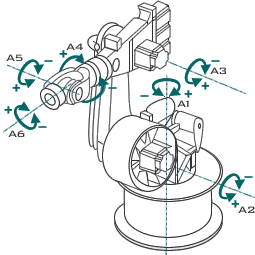
\includegraphics[height=.187\textheight]{robots/articulated-robot}
		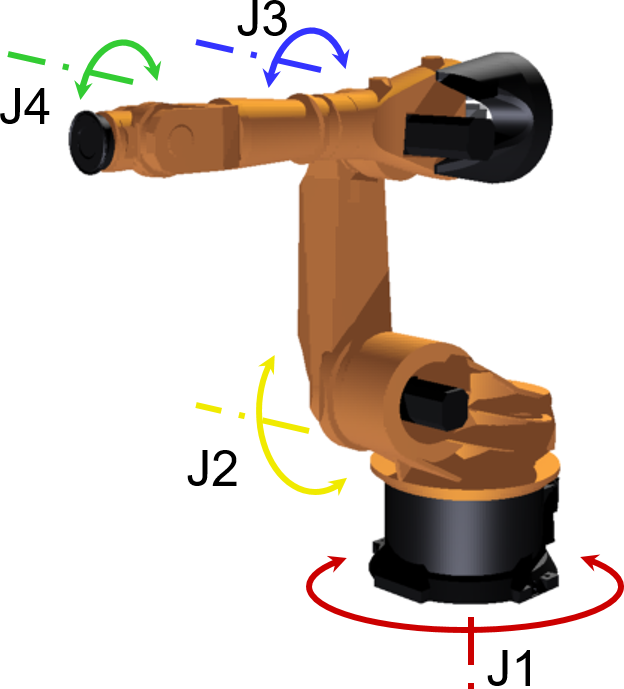
\includegraphics[height=.187\textheight]{robots/articulated-robot-model}}
		{\caption[Diagrams of an articulated robot]{Diagrams of an articulated robot\protect\footnotemark}\label{fig:articulated-robot}}

		\ffigbox[\FBwidth]
		{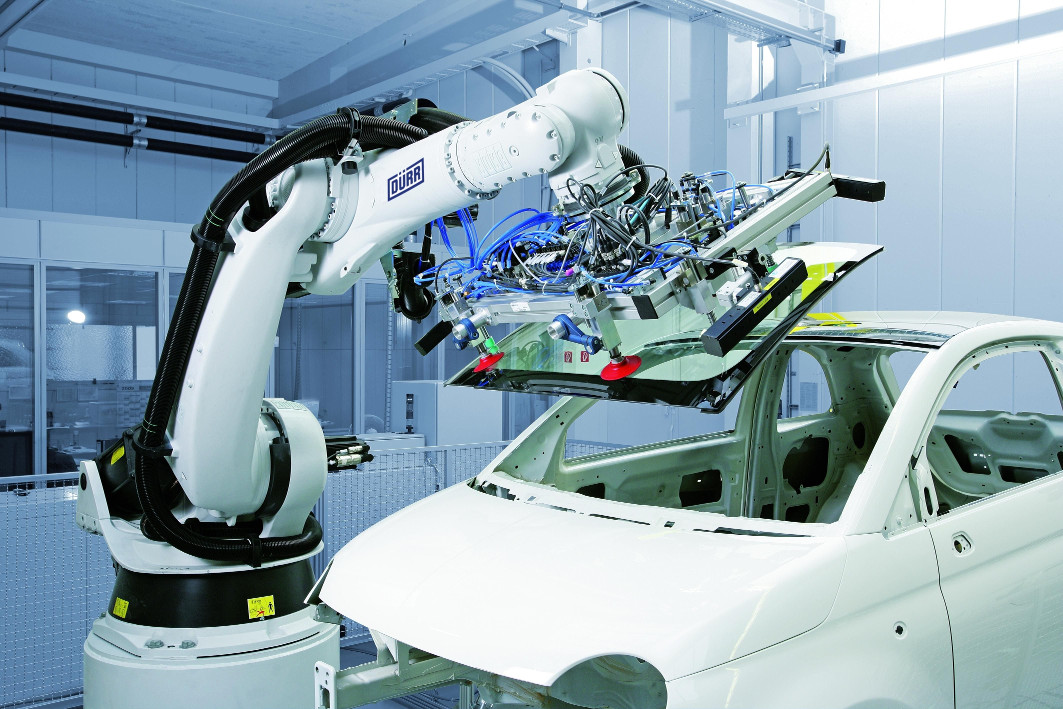
\includegraphics[height=.187\textheight]{robots/articulated-robot-kuka}}
		{\caption[Articulated  robot installing a windshield in a car]{Articulated  robot installing a windshield in a car\protect\footnotemark}\label{fig:articulated-robot-kuka}}
	\end{floatrow}
\end{figure}
\footnotetext[\the\numexpr\value{footnote}-1\relax]{\url{http://slideplayer.com/slide/7362200}}
\footnotetext[\value{footnote}]{\url{http://gracemarketdata.com/index.php/component/virtuemart/2001-detail}}



\subsection{Collaborative robotic arms}

Collaborative robots are usually articulated robotic arms that were designed to be safe \cite{Haddadin2011,Ceriani2014} to operate around humans. They typically move at low velocities and have force-torque / motor current sensors along with enclosure in pressure / capacitive sensitive materials in order to detect collisions and stop the robot movement before injuring humans. Other safety measures rely on the usage of elastic actuators and soft padding to attenuate the impact damage while complementary measures include the detection of approaching humans / objects using \glspl{lidar} / RGB-D sensors in order to reduce the robot operation velocity and adjust the trajectory to avoid collisions. In \cref{fig:collaborative-robots-t1,fig:collaborative-robots-t2} it is presented an overview of the main collaborative robots currently available along with the specification of their main hardware characteristics and targeted applications.

%Articles:\\
%- Collaborative robot - Robotiq ebook | Mathieu2015
%- Dual arm manipulation - A survey | Smith2012
%- A brief survey of commercial robotic arms for research on manipulation | Lu2012
%- Survey of robotic arm and parameters | Patidar2016


\begin{table}[H]
	\centering
	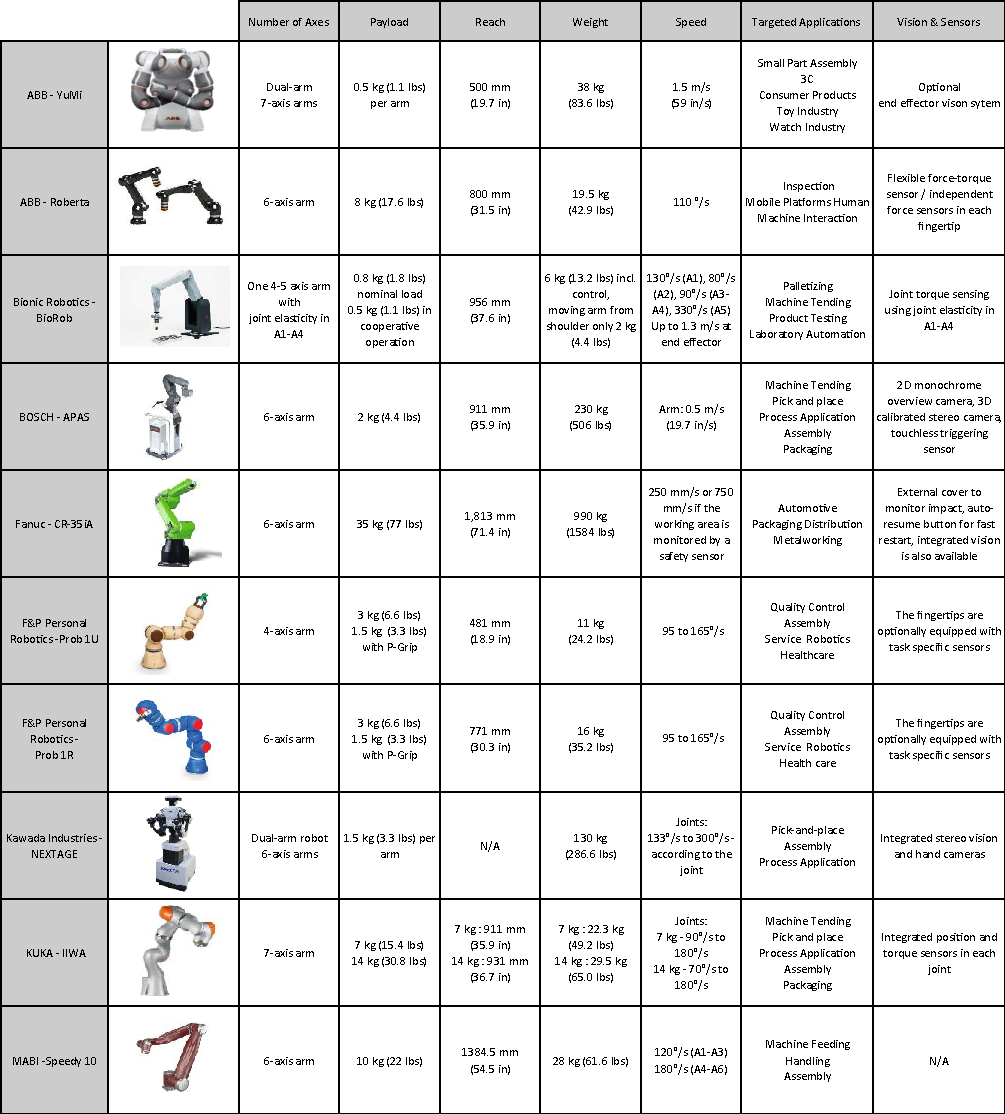
\includegraphics[width=\linewidth]{robots/collaborative-robots-t1}
	\caption[Collaborative robots (a)]{Collaborative robots (a) \cite{Mathieu2015}}
	\label{fig:collaborative-robots-t1}
\end{table}

\begin{table}[H]
	\centering
	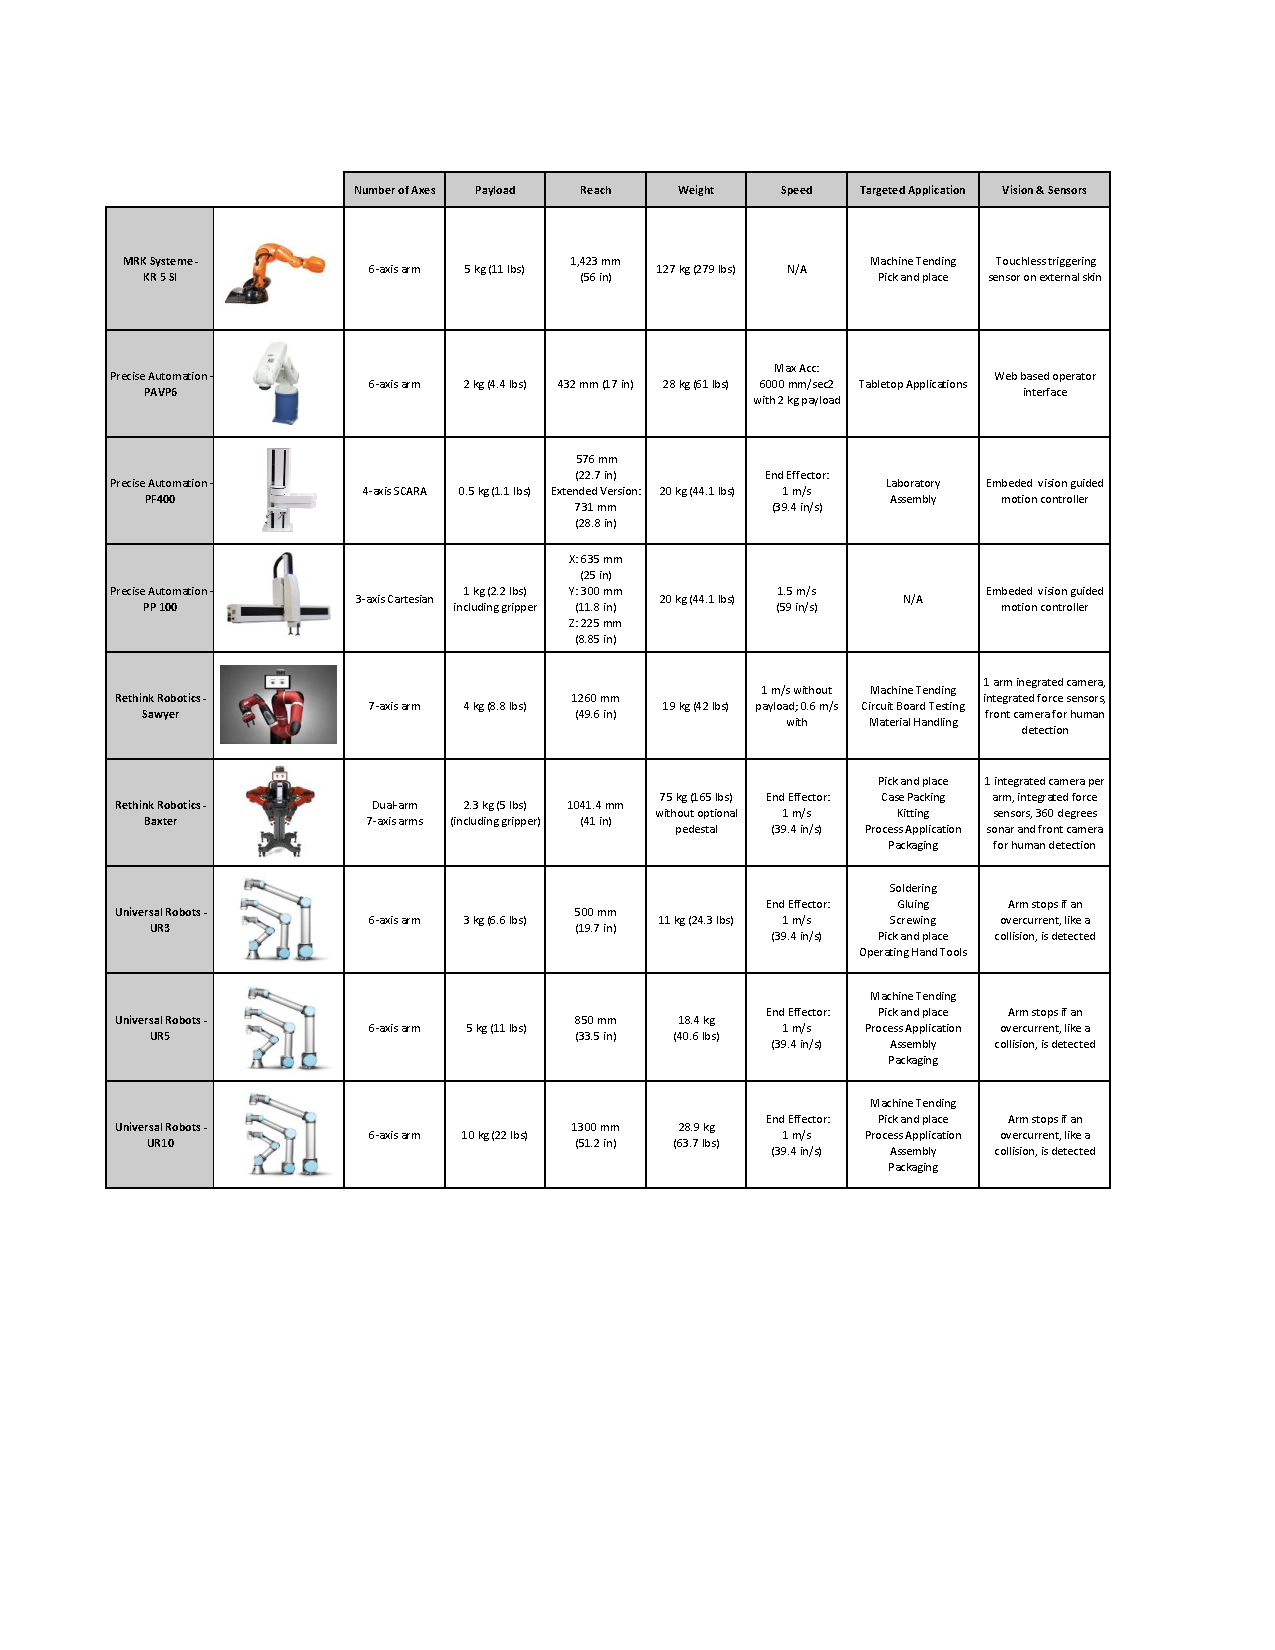
\includegraphics[width=\linewidth]{robots/collaborative-robots-t2}
	\caption[Collaborative robots (b)]{Collaborative robots (b) \cite{Mathieu2015}}
	\label{fig:collaborative-robots-t2}
\end{table}


\section{Robotic end effectors}

End effectors are hardware devices attached at the end of robotic arms in order to allow them to interact with the environment. This interaction can be passive if the end effectors are only comprised of sensors (used for inspection, quality assurance, surveillance) or can be active in which the robot physically interacts with the environment.

Grippers are one the most complex active end effectors given their need to grasp \cite{Sahbani2012} and hold a wide range of objects with different size, shape, weight and stiffness. They are also one of the most flexible and versatile end effector given that they can be used to handle a wide range of objects when performing very different tasks. The remaining end effectors are usually tailored for very specific tasks (for example welding, cutting, drilling, screwing, grinding, painting, among many others).

The following list presents a brief overview of the main end effectors currently available.

\begin{itemize}
	\item Grippers
	\begin{itemize}
		\item Impactive grippers
		\begin{itemize}
			\item Parallel fingers
			\item Angular fingers
			\item Universal grippers (for example the Versaball)
			\item Anthropomorphic grippers with 5 fingers
		\end{itemize}
		\item Astrictive grippers
		\begin{itemize}
			\item Vacuum grippers
			\item Bernoulli grippers
			\item Magnetic grippers
			\item Electrostatic grippers
		\end{itemize}
		\item Contigutive grippers
		\begin{itemize}
			\item Chemical adhesion grippers
			\item Thermal adhesion grippers
		\end{itemize}
		\item Ingressive grippers
		\begin{itemize}
			\item Hooks
			\item Loops
		\end{itemize}
	\end{itemize}
	\item Perception sensors
	\begin{itemize}
		\item 2D / \gls{tof} cameras
		\item Point / line lasers
		\item \glspl{lidar}
		\item RGB-D sensors
		\item Structured light sensors
	\end{itemize}
	\item Collision sensors
	\item Force-torque sensors
	\item Projectors (\gls{dlp} / galvanometers)
	\item Welding torches
	\item Cutting tools
	\item Drilling tools
	\item Milling tools
	\item Grinders
	\item Sanders
	\item Polishers
	\item Finishers
	\item Sprayers
	\item Screw drivers
	\item Spanners
	\item Ladles
\end{itemize}


For assembly operations the most useful end effectors are the grippers, perception / force-torque sensors and specialized tools (screw drivers, spanners, welders, among others). Most object manipulation tasks can be done with grippers with two or three fingers (examples in \cref{fig:yumi-gripper-vamera-vacuum,fig:schunk-parallel-grippers,fig:schunk-angular-gripper,fig:schunk-self-centering-gripper}) or with adaptive two / three finger grippers (examples in \cref{fig:robotiq-adaptive-2-finger-gripper,fig:robotiq-adaptive-3-finger-gripper}). For tasks that require coarse accuracy, magnetic / vacuum grippers (examples in \cref{fig:zimmer-magnetic-gripper,fig:schunk-vacuum-gripper,fig:schmalz-vacuum-area-gripper}) might be a suitable alternative. For difficult to grasp objects, flexible grippers (such as the ones shown in \cref{fig:versa-ball,fig:festo-multichoice-gripper}) provide a robust approach. For very complex tasks that may require advanced dexterity, anthropomorphic grippers \cite{Amor2012,Mattar2013} (example in \cref{fig:schunk-svh-hand}) offer a very advanced solution.

\begin{figure}[H]
	\begin{floatrow}[4]
		\ffigbox[1.1\FBwidth]
		{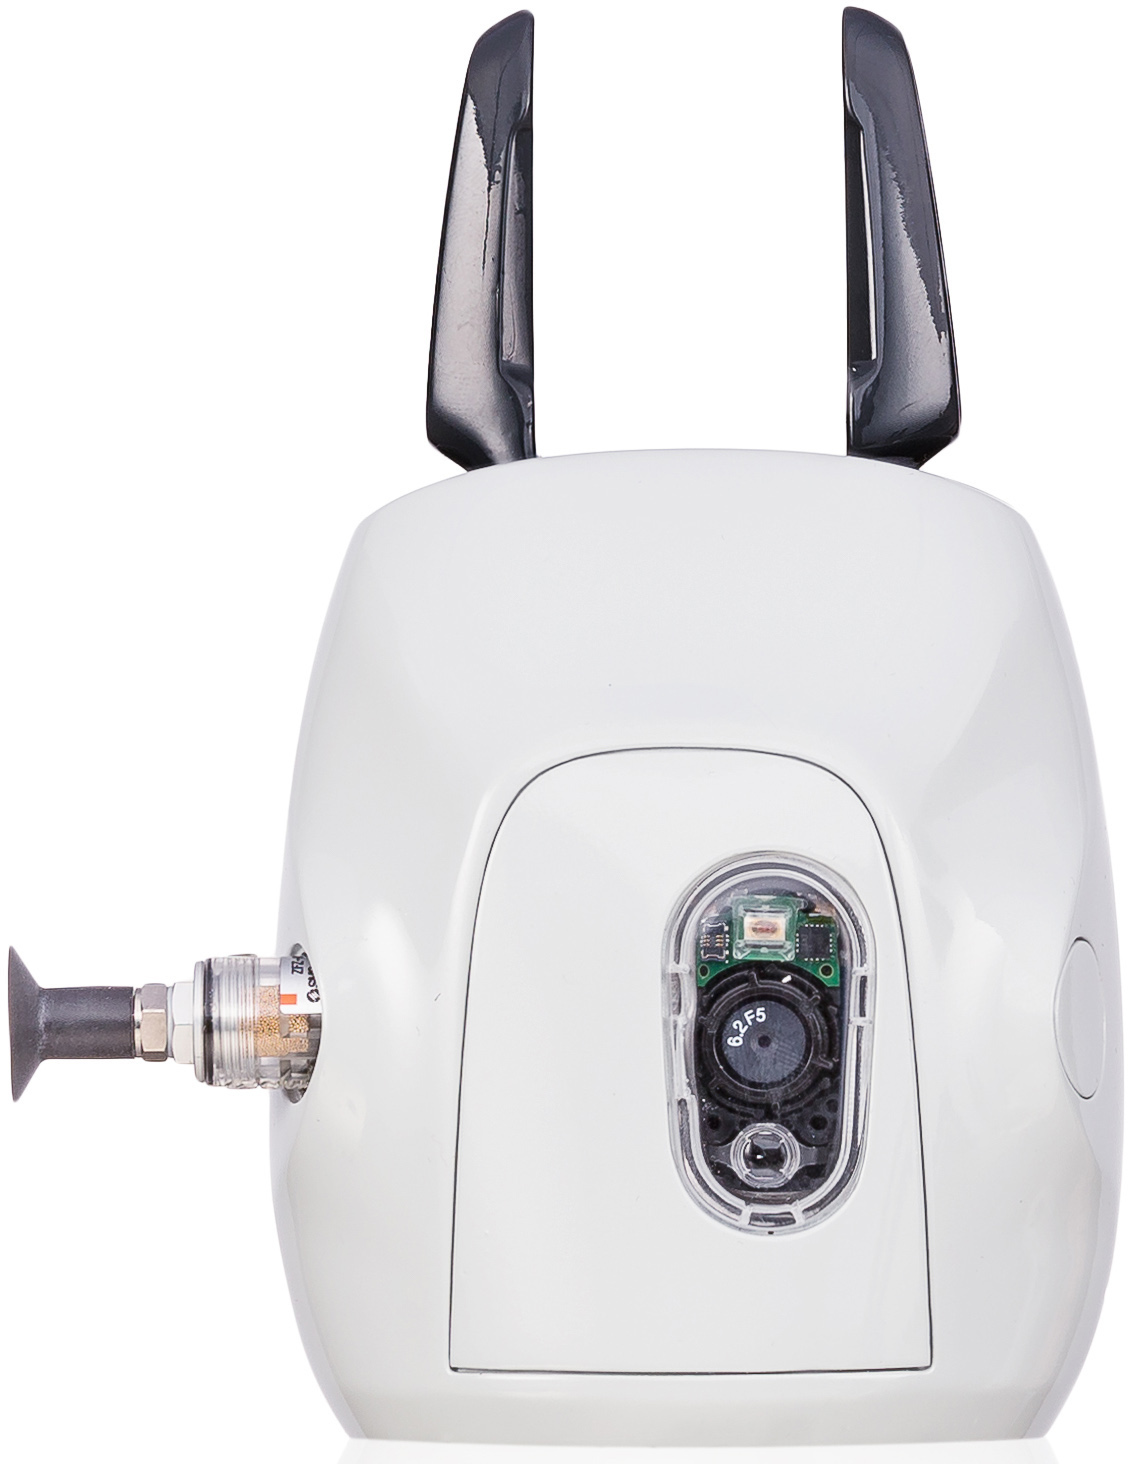
\includegraphics[height=.19\textheight]{grippers/yumi-gripper-vamera-vacuum}}
		{\caption[ABB Yumi dual finger / vacuum / camera gripper]{ABB Yumi dual finger / vacuum / camera gripper \protect\footnotemark}\label{fig:yumi-gripper-vamera-vacuum}}

		\ffigbox[1.1\FBwidth]
		{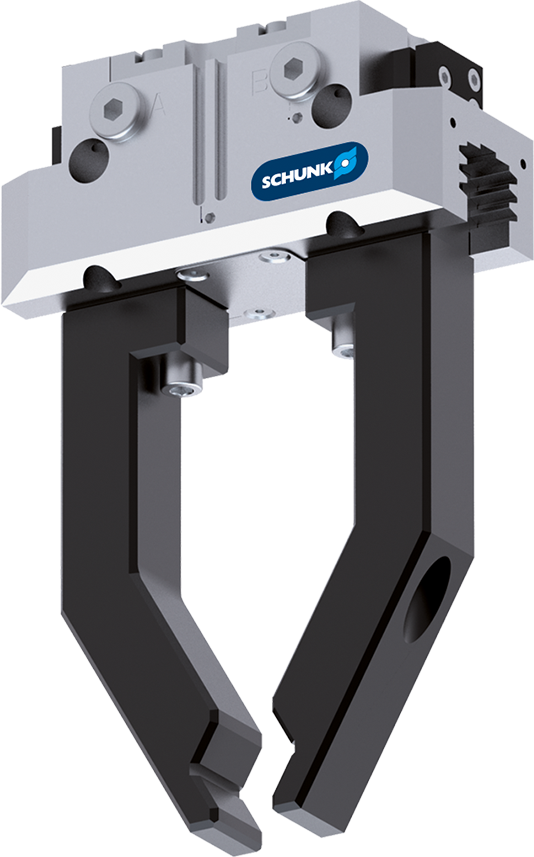
\includegraphics[height=.19\textheight]{grippers/schunk-parallel}}
		{\caption[Schunk parallel gripper]{Schunk parallel gripper\protect\footnotemark}\label{fig:schunk-parallel-grippers}}

		\ffigbox[1.1\FBwidth]
		{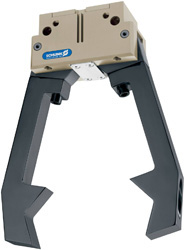
\includegraphics[height=.19\textheight]{grippers/schunk-angular-gripper}}
		{\caption[Schunk angular gripper]{Schunk angular gripper\protect\footnotemark}\label{fig:schunk-angular-gripper}}

		\ffigbox[1.1\FBwidth]
		{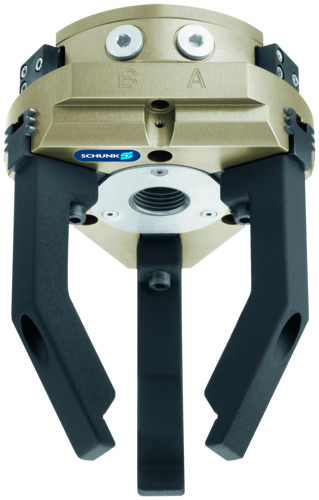
\includegraphics[height=.19\textheight]{grippers/schunk-self-centering-gripper}}
		{\caption[Schunk self-centering gripper]{Schunk self-centering gripper\protect\footnotemark}\label{fig:schunk-self-centering-gripper}}
	\end{floatrow}
\end{figure}
\footnotetext[\the\numexpr\value{footnote}-3\relax]{\url{http://new.abb.com/products/robotics/yumi}}
\footnotetext[\the\numexpr\value{footnote}-2\relax]{\url{https://us.schunk.com/us_en/home/pgn-plus-p}}
\footnotetext[\the\numexpr\value{footnote}-1\relax]{\url{https://us.schunk.com/us_en/gripping-systems/\#/series/pwg-plus}}
\footnotetext[\value{footnote}]{\url{https://us.schunk.com/us_en/gripping-systems/\#/series/pzb-plus}}


\begin{figure}[H]
	\begin{floatrow}[4]
		\ffigbox[1.05\FBwidth]
		{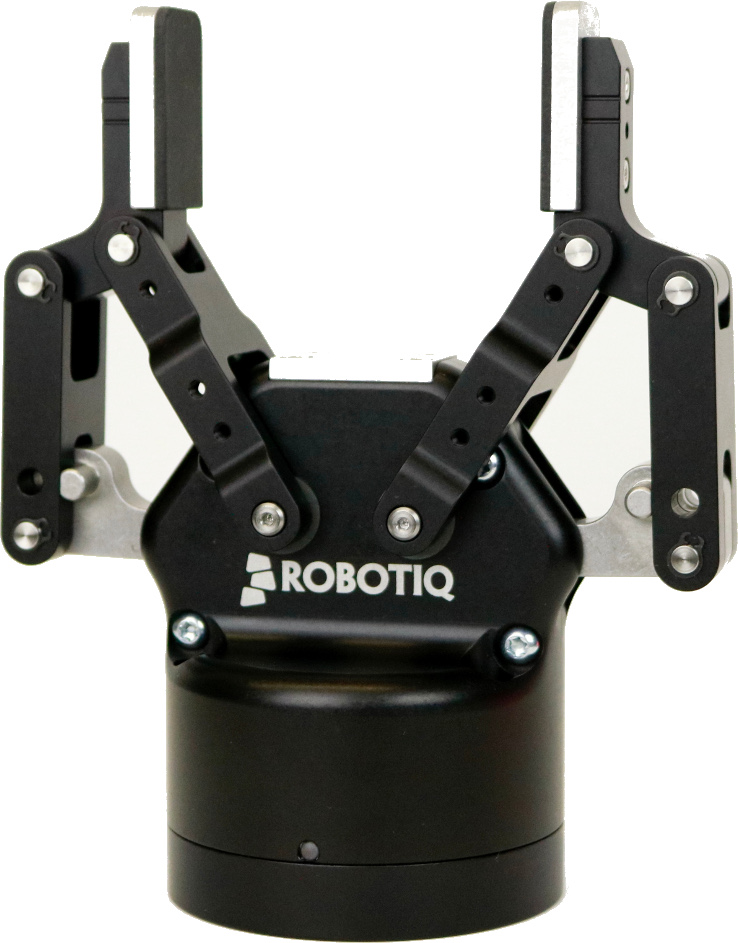
\includegraphics[height=.17\textheight]{grippers/robotiq-adaptive-2-finger-gripper}}
		{\caption[Robotiq adaptive 2 finger gripper]{Robotiq adaptive 2 finger gripper\protect\footnotemark}\label{fig:robotiq-adaptive-2-finger-gripper}}

		\ffigbox[1.05\FBwidth]
		{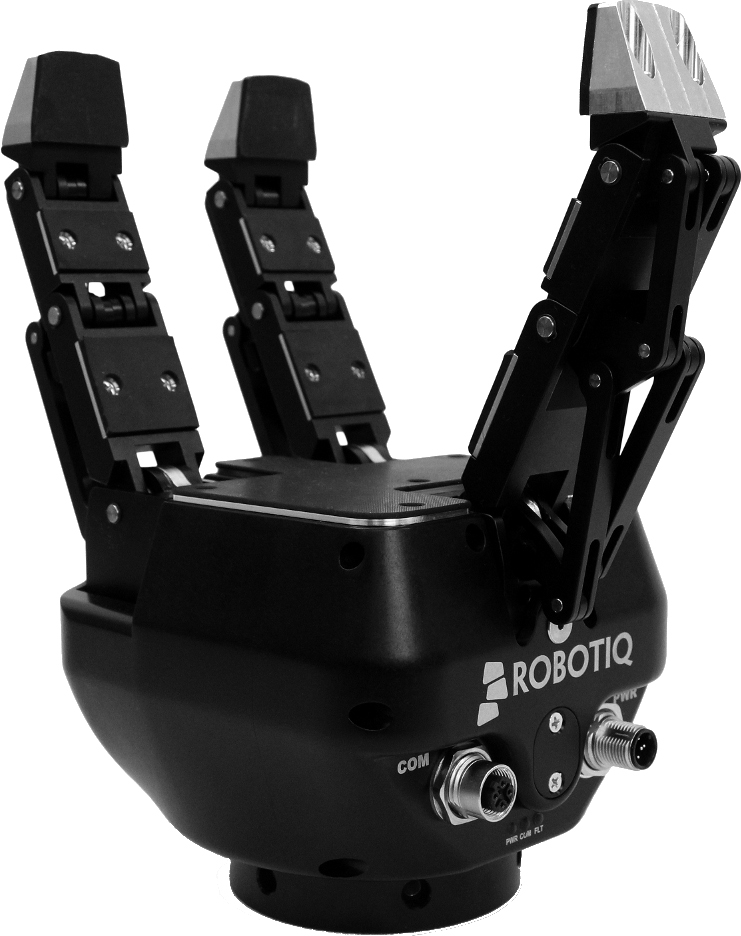
\includegraphics[height=.17\textheight]{grippers/robotiq-adaptive-3-finger-gripper}}
		{\caption[Robotiq adaptive 3 finger gripper]{Robotiq adaptive 3 finger gripper\protect\footnotemark}\label{fig:robotiq-adaptive-3-finger-gripper}}

		\ffigbox[1.05\FBwidth]
		{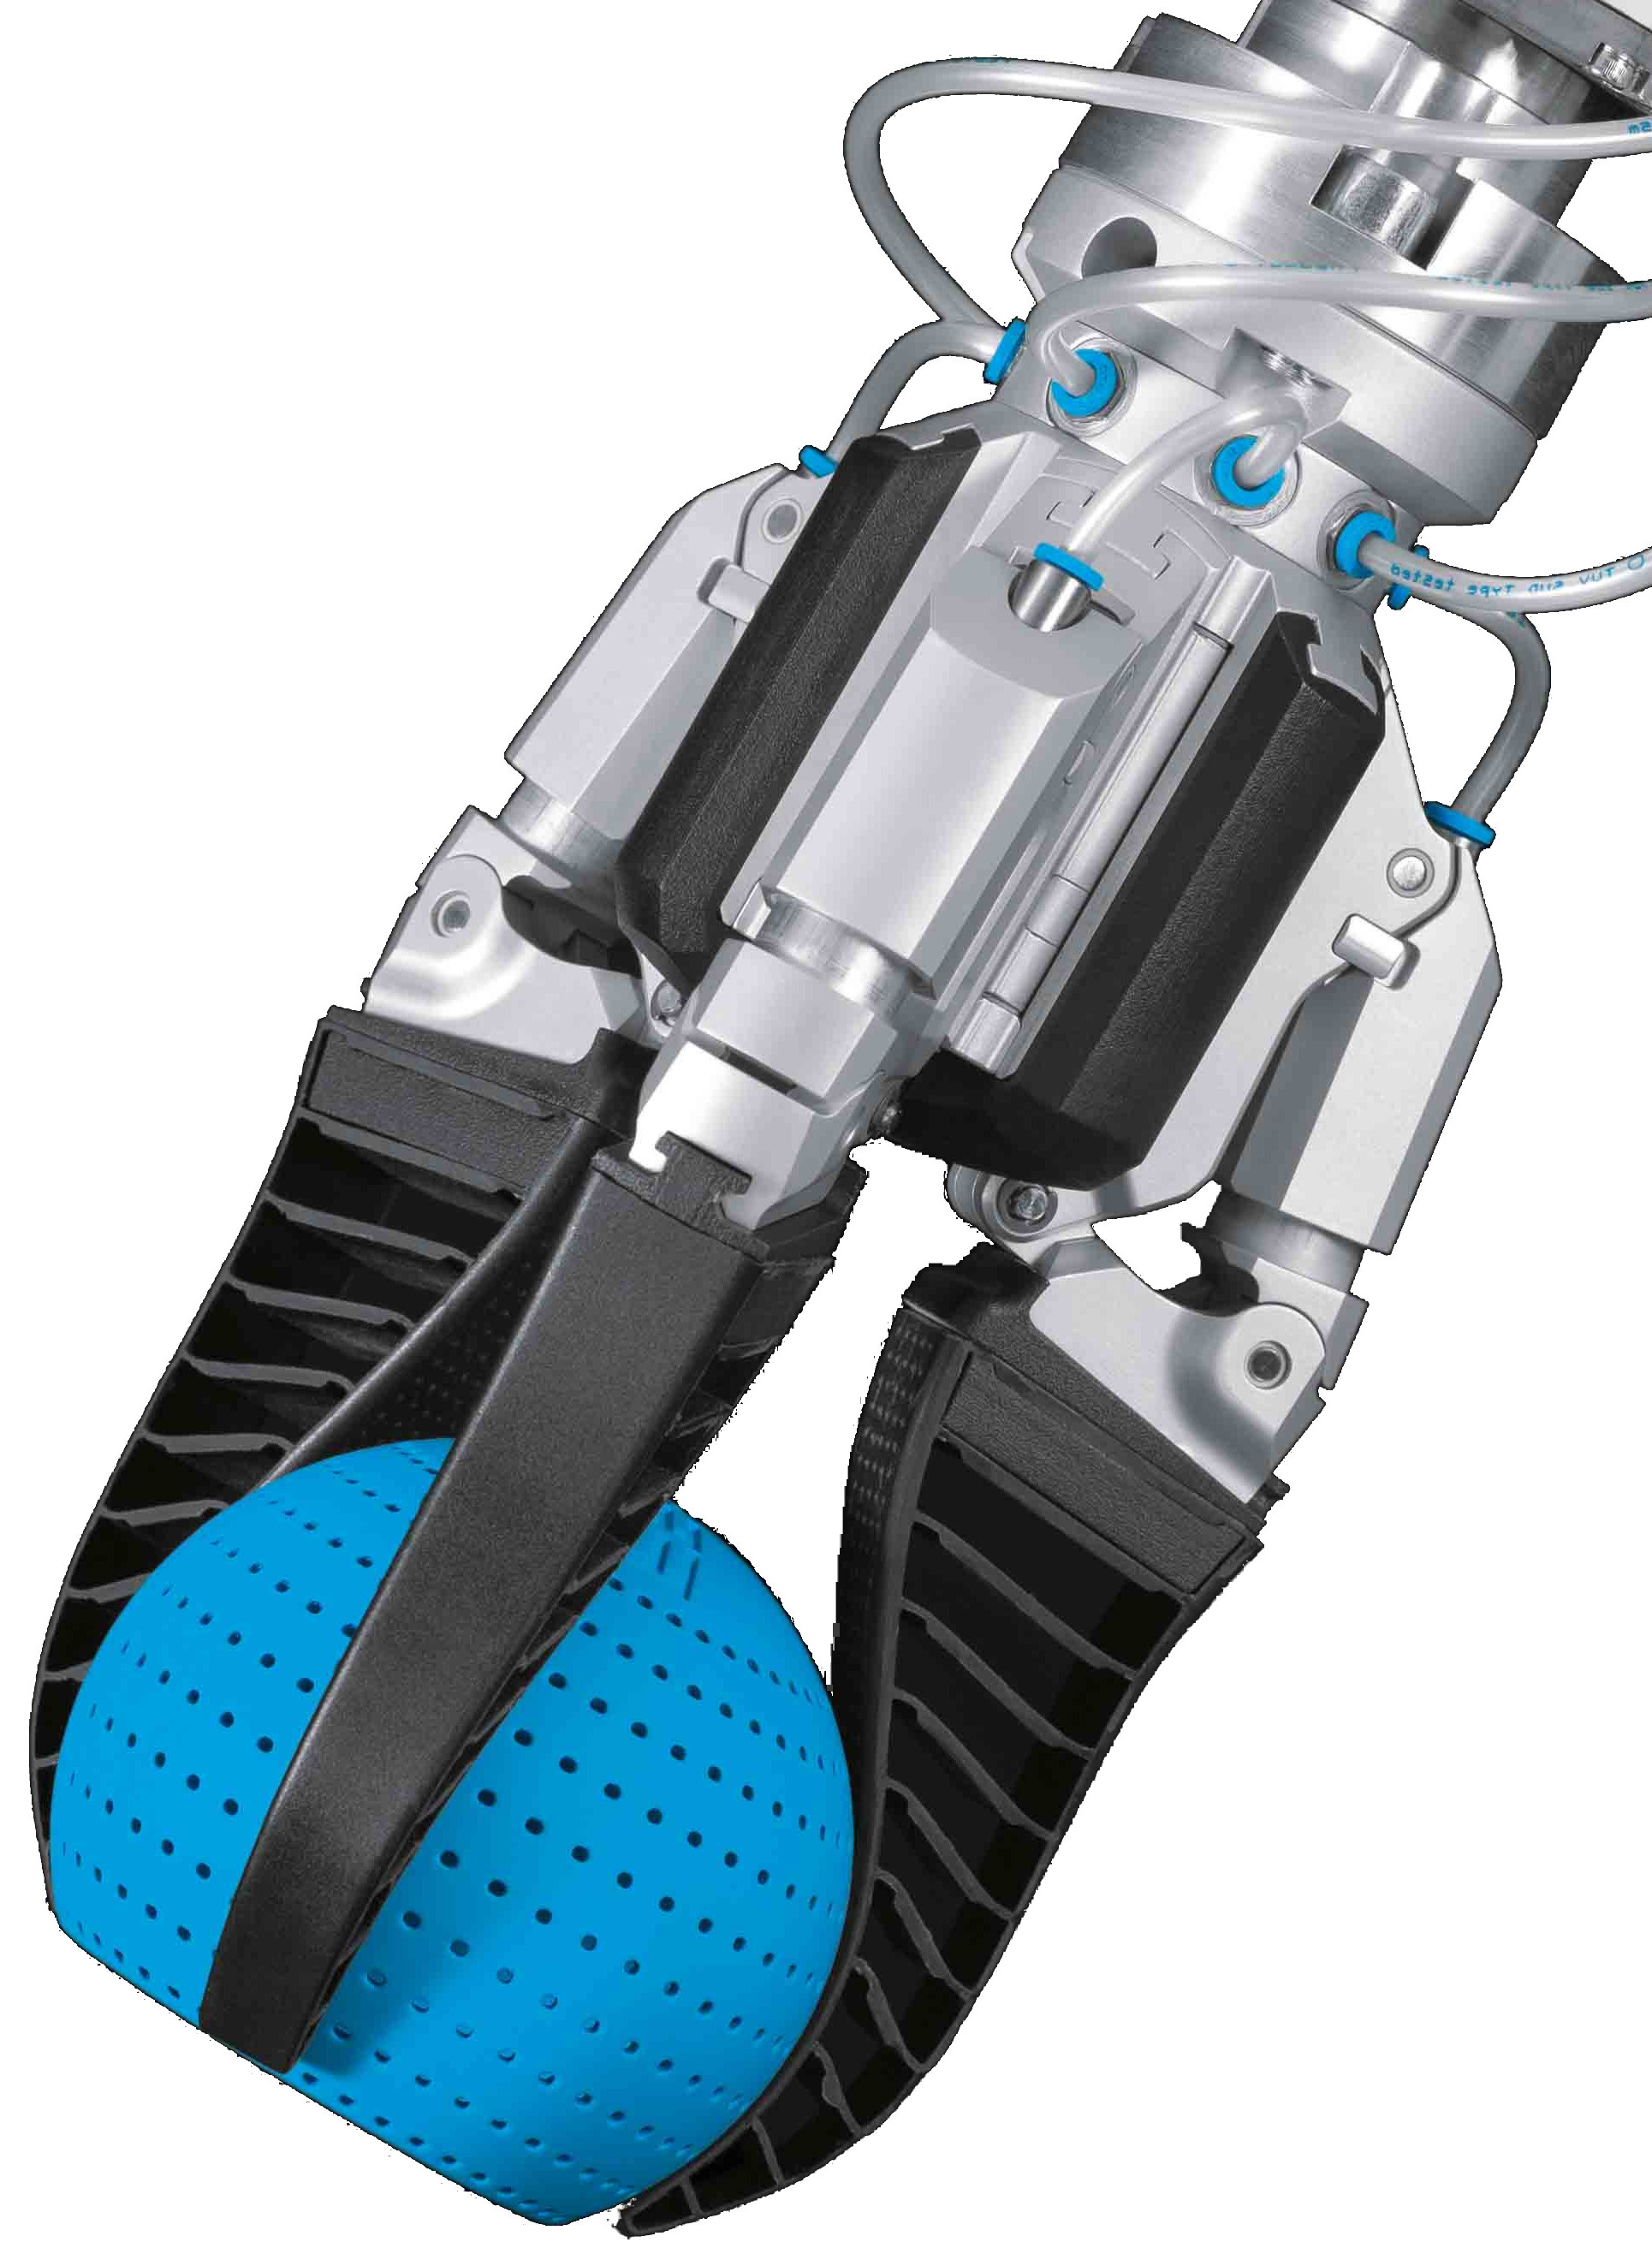
\includegraphics[height=.17\textheight]{grippers/festo-multichoice-gripper}}
		{\caption[Festo flexible 3 finger gripper]{Festo flexible 3 finger gripper\protect\footnotemark}\label{fig:festo-multichoice-gripper}}

		\ffigbox[1\FBwidth]
		{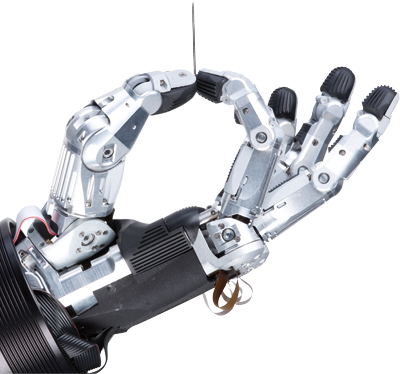
\includegraphics[height=.17\textheight]{grippers/schunk-svh-precision-grip}}
		{\caption[Schunk anthropomorphic gripper]{Schunk anthropomorphic gripper\protect\footnotemark}\label{fig:schunk-svh-hand}}
	\end{floatrow}
\end{figure}
\footnotetext[\the\numexpr\value{footnote}-3\relax]{\url{http://blog.robotiq.com/topic/2-finger-robot-gripper}}
\footnotetext[\the\numexpr\value{footnote}-2\relax]{\url{http://support.robotiq.com/display/IMB/Home}}
\footnotetext[\the\numexpr\value{footnote}-1\relax]{\url{https://www.festo.com/group/en/cms/10221.htm}}
\footnotetext[\value{footnote}]{\url{http://mobile.schunk-microsite.com/en/produkte/products/servo-electric-5-finger-gripping-hand-svh.html}}


\begin{figure}[H]
	\begin{floatrow}[4]
		\ffigbox[2.4\FBwidth]
		{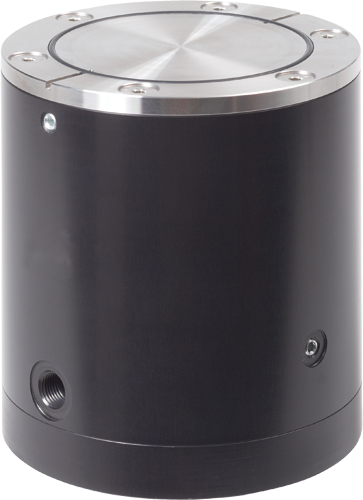
\includegraphics[height=.08\textheight]{grippers/zimmer-magnetic-gripper}}
		{\caption[Zimmer magnetic gripper]{Zimmer magnetic gripper\protect\footnotemark}\label{fig:zimmer-magnetic-gripper}}

		\ffigbox[1.98\FBwidth]
		{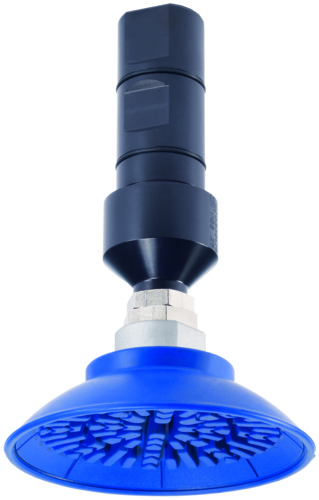
\includegraphics[height=.11\textheight]{grippers/schunk-vacuum-gripper}}
		{\caption[Schunk vacuum gripper]{Schunk vacuum gripper\protect\footnotemark}\label{fig:schunk-vacuum-gripper}}

		\ffigbox[2\FBwidth]
		{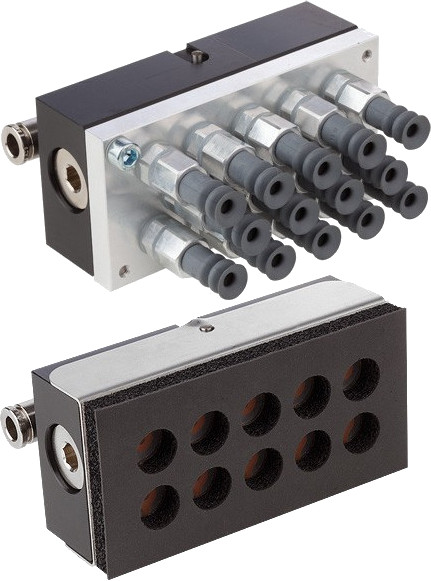
\includegraphics[height=.1\textheight]{grippers/schmalz-vacuum-area-gripper}}
		{\caption[Schmalz vacuum area gripper]{Schmalz vacuum area gripper\protect\footnotemark}\label{fig:schmalz-vacuum-area-gripper}}

		\ffigbox[\FBwidth]
		{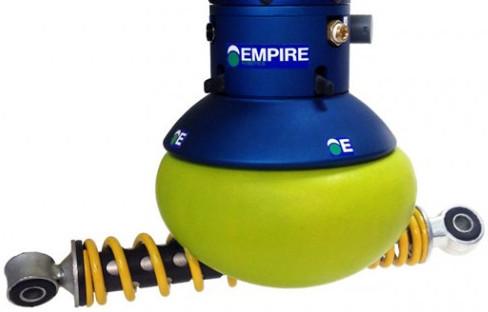
\includegraphics[height=.11\textheight]{grippers/versa-ball}}
		{\caption[Versa ball]{Versa ball\protect\footnotemark}\label{fig:versa-ball}}
	\end{floatrow}
\end{figure}
\footnotetext[\the\numexpr\value{footnote}-3\relax]{\url{http://www.zimmer-group.de/en/ajax/productdetail?struktkey=\%24MN-SOM-\%24PLC-V-\%24PG-GRE-\%24SR-HM1000&productkey=HM1097NC&layout=1}}
\footnotetext[\the\numexpr\value{footnote}-2\relax]{\url{http://de.schunk.com/de_en/gripping-systems/\#/series/gsw-v}}
\footnotetext[\the\numexpr\value{footnote}-1\relax]{\url{https://www.schmalz.com/en/vacuum-technology-for-automation/vacuum-components/area-gripping-systems-and-end-effectors}}
\footnotetext[\value{footnote}]{\url{http://www.extremetech.com/extreme/174723-soft-robotic-gripper-uses-vacuum-pressure-and-a-beanbag-to-move-objects}}

%Articles:\\
%- An overview of 3D object grasp synthesis algorithms
%- A review on importance of universal gripper in industrial robot applications
%- A survey of bio-inspired robotics hands implementation - New directions in dexterous manipulation

%Articles:\\
%- An Adaptive Feedback Scheduling Algorithm for Robot Assembly and Real-Time Control Systems


\section{Automatic tool change}

Given the wide variety of objects that assembly operations may require, automatic tool change devices (such as the one shown in \cref{fig:tool-changer}) are very useful to allow the robot to autonomously change the end effector in order to perform the current task with the most appropriate hardware configuration.

\begin{figure}[H]
	\centering
	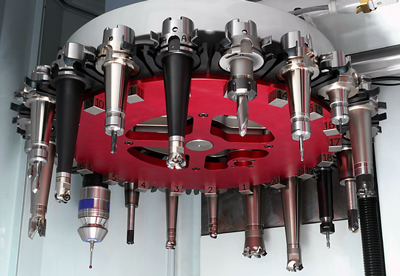
\includegraphics[width=0.66\linewidth]{grippers/tool-changer}
	\caption[Automatic tool changer with 20 different robotic arm end effectors]{Automatic tool changer with 20 different robotic arm end effectors\protect\footnotemark}
	\label{fig:tool-changer}
\end{figure}
\footnotetext{\url{http://www.h-h.com.au/ae_mc_tool-changer.htm}}


\section{Environment fixtures}

Environment fixtures are a very useful approach to ensure that the assembly objects are provided by the human operator at known positions with high accuracy (avoiding complex perception systems). These fixtures can be in the form of packaging trays (example in \cref{fig:vacuum-formed-packaging-trays}) allowing quick restock of assembly objects or can be inclined loading docks (example in \cref{fig:parts-loading-fixture}), in which the human operators insert the assembly objects at the top and robot removes them always at the same place at the bottom (when the robot removes one object the gravity pulls the next one into place).

Another useful application of environment fixtures is for temporarily holding the assembly objects, either using static fixtures (examples in \cref{fig:profile-vertical-fixture,fig:profile-horizontal-fixture}) or actuated grippers (example in \cref{fig:part-fixture-actuated}). This can be very useful to allow assembly operations with only one robotic arm and also for changing gripping positions of grasped objects (examples in \cref{fig:part-fixture-actuated} and \cite{Chavan2015}).

%Articles:\\
%- Prehensile Pushing - In-hand Manipulation with Push-Primitives | Chavan2015

\begin{figure}[H]
	\begin{floatrow}[2]
		\ffigbox[\FBwidth]
		{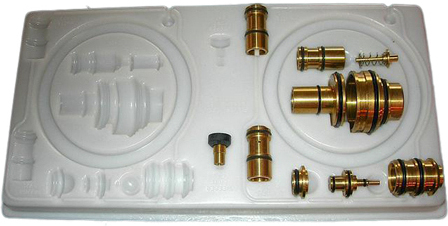
\includegraphics[height=.183\textheight]{grasping/vacuum-formed-packaging-trays}}
		{\caption[Vacuum formed packaging tray]{Vacuum formed packaging tray\protect\footnotemark}\label{fig:vacuum-formed-packaging-trays}}

		\ffigbox[\FBwidth]
		{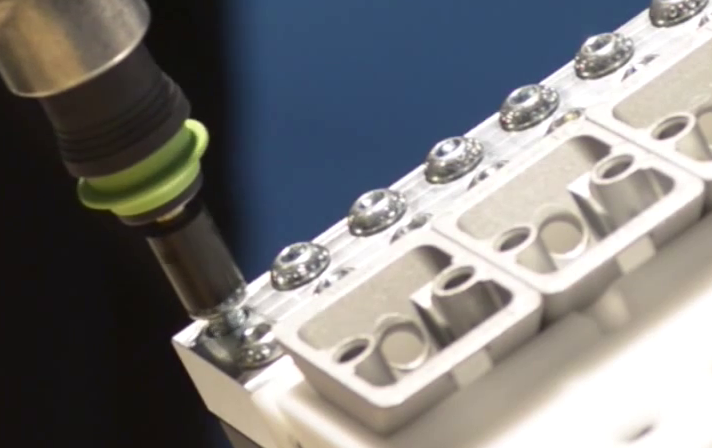
\includegraphics[height=.183\textheight]{grasping/parts-loading-fixture}}
		{\caption[Parts loading dock]{Parts loading dock\protect\footnotemark}\label{fig:parts-loading-fixture}}
	\end{floatrow}
\end{figure}
\footnotetext[\the\numexpr\value{footnote}-1\relax]{\url{http://www.vinayakapolyproducts.com/vacuum-formed-packaging-trays-2186055.html}}
\footnotetext[\value{footnote}]{\url{https://www.youtube.com/watch?v=2jYhdmk-pMg}}

\begin{figure}[H]
	\begin{floatrow}[3]
		\ffigbox[\FBwidth]
		{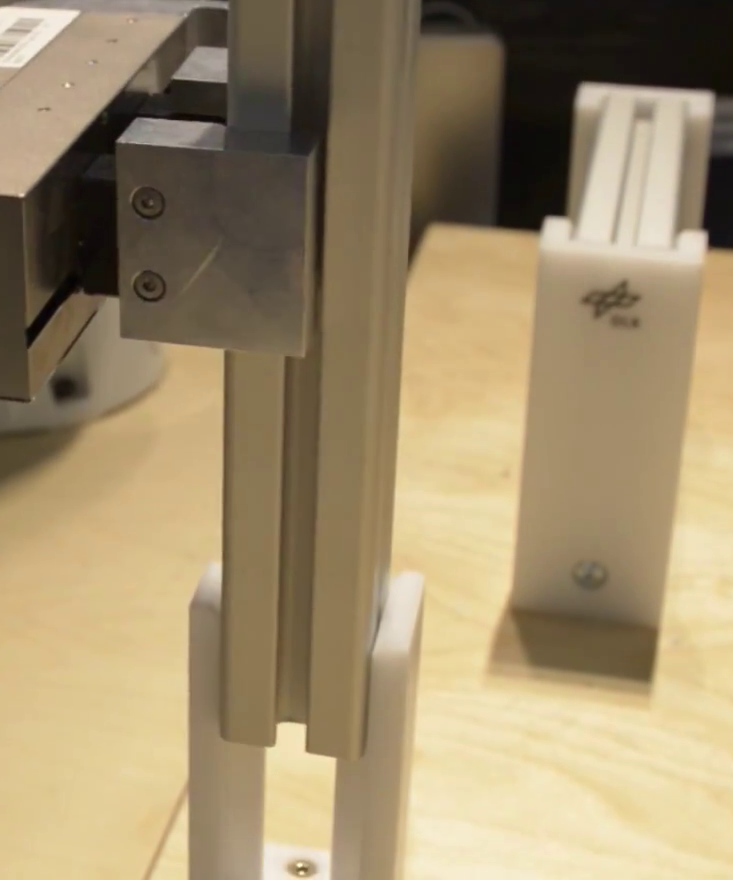
\includegraphics[height=.22\textheight]{grasping/profile-vertical-fixture}}
		{\caption[Aluminum profile vertical fixture]{Aluminum profile vertical fixture\protect\footnotemark[\value{footnote}]}\label{fig:profile-vertical-fixture}}

		\ffigbox[\FBwidth]
		{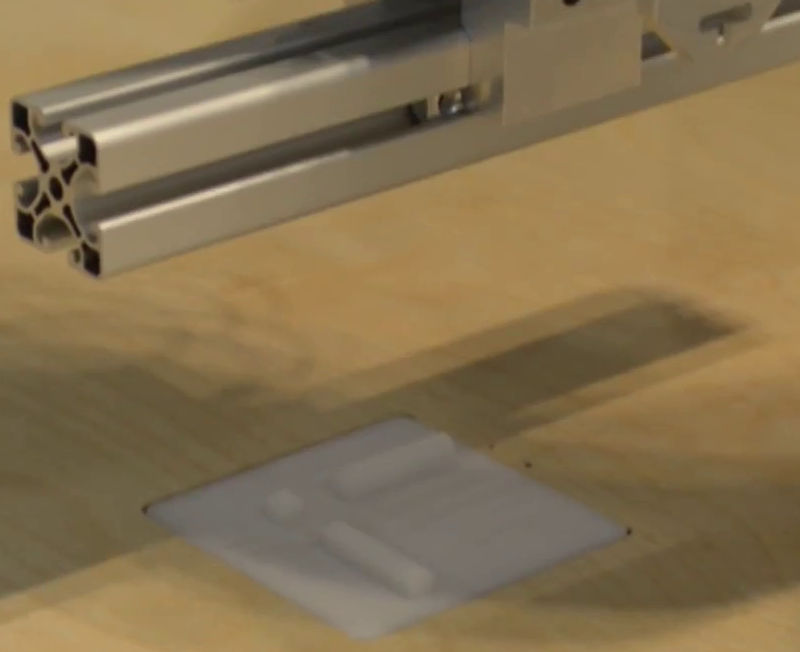
\includegraphics[height=.22\textheight]{grasping/profile-horizontal-fixture}}
		{\caption[Aluminum profile horizontal fixture]{Aluminum profile horizontal fixture\protect\footnotemark[\value{footnote}]}\label{fig:profile-horizontal-fixture}}

		\ffigbox[\FBwidth]
		{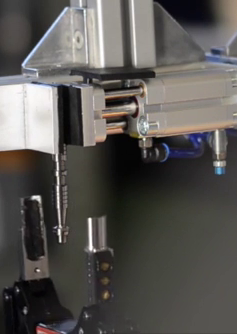
\includegraphics[height=.22\textheight]{grasping/part-fixture-actuated}}
		{\caption[Actuated object holder]{Actuated object holder\protect\footnotemark}\label{fig:part-fixture-actuated}}
	\end{floatrow}
\end{figure}
\footnotetext[\value{footnote}]{\url{https://www.youtube.com/watch?v=MuKOPnrYS-Q}}



\section{Alignment devices}

Assembling objects is a very complex task that requires accurate perception and pose estimation of the assembly parts and also proper gripping positioning. For interconnected objects, force-torque sensors and alignment devices such as \glspl{rcc} (example in \cref{fig:remote-center-compensator}) can be very useful tools for tolerating small misalignments and ensuring proper part installation.

\begin{figure}[H]
	\centering
	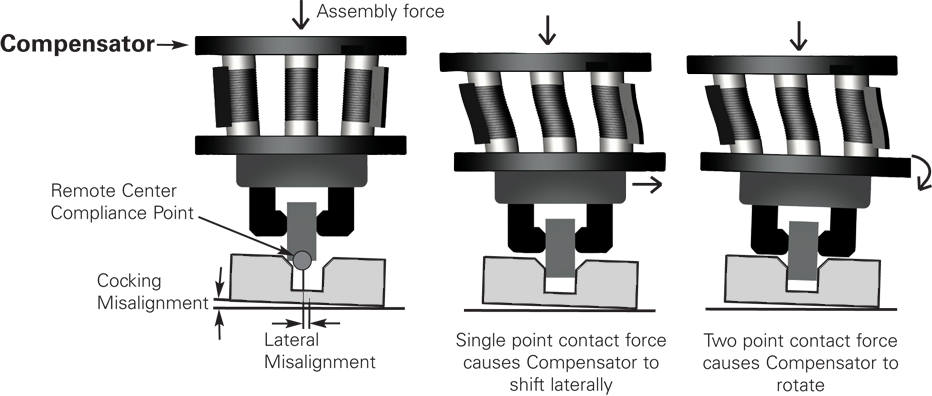
\includegraphics[width=0.88\linewidth]{grasping/remote-center-compensator}
	\caption[Usage of a \glsentrytext{rcc} to tolerate slight part misalignments]{Usage of a \glsentrytext{rcc} to tolerate slight part misalignments\protect\footnotemark}
	\label{fig:remote-center-compensator}
\end{figure}
\footnotetext{\url{http://www.ati-ia.com/products/compliance/Compensator_product_desc.aspx}}

